\chapter{Case}
%%%%%%%%%%
This chapter serves to connect the scientific background and methodology with the research project. 
It sheds light into the organizational environment, which will be starting point for reference model construction.  

\section{Organizational Setting}
This thesis comes into being as part of the \textit{ERCIS Omni-channel lab powered by Arvato}. This cooperation fosters research in omni-channel CRM through cooperation with Arvato, a leading European outsourcing provider. The focus is set on the CRM services division, which is one of four 
solution groups. While the German market has the largest share, Arvato operates international. The organizational structure can be described as decentralized in the past, but it is intended to integrate the independent country organizations more deeply within the solution group. As clients intensify international outsourcing of customer services to Arvato, a need to deliver an orchestrated outsourcing concept across borders arises. The solution group CRM therefore needs more alignment in their three constituents

\begin{itemize}
	\item Sales \& Business Development,
	\item Portfolio Management \& IT and
	\item Operations.
\end{itemize}

An investigation in organizational structures is not in scope of this work, but this view on the business helps to derive a process structure. As an analogy to the domain of retail, one can see its supply and distribution side in form of Sales \& Business Development and Operations, respectively. The \textit{Sales \& Business Development }organization is oriented towards the outsourcing company, e.g., client. It is the main channel of communication to manage existing and potential clients and hence enables the \textit{supply} of outsourcing contracts and therefore business to the organization.\\
 \textit{Portfolio Management \& IT} organizes available service products and their technological foundation. Especially CRM platforms, their selection and implementation is part of its capabilities. With a decentralized orientation in the past, Arvato faces the problem of a heterogeneous system landscape in client businesses, as there was no guidance for platform selection. The aspired product orientation at Arvato demands standardization in platforms, so that a managed portfolio becomes necessary. As it is a characteristic of CRM outsourcing that clients dictate parts of the environment, \eg, technology or processes, a BPO provider needs to be flexible to react to these requirements. Interface to Sales \& Business Development are the product portfolio, which is marketed to the client. In addition, it supports in design and instantiation of products for a specific client. An internal view of product constituents, namely people, process and platform, is directed towards implementation of services and their operational use. 
  \textit{Operations}, on the distribution side in the retail analogy, is oriented towards the customer. With call center business as core of BPO in CRM, it becomes clear that human resources are one key ingredient of the service delivery.  \\
  
  Drawing from the three described constituents of the Arvato CRM solution group, one can identify three stakeholders in the BPO provider organization. Recalling the BPO Outsourcing chain (\Fig \ref{fig:bpochain}), one part of the provider is linked to the client, another to the customer and the third is located in the center. Applying this logic to the three aforementioned units of Arvato CRM and taking a perspective that is scoped on the essential task of the unit, Sales \& Business Development targets clients and Operations is oriented towards the customers. Distancing from Arvato terminology, one can name these two stakeholders simply \textit{Sales} and \textit{Operations}. \\
  
  Portfolio Management \& IT influences both sides, as well as it acts between the two interfaces. Besides, the central part of the chain can be used to model the stakes of the BPO provider as a whole. With the taken perspective that factors out coordinating activities in the three units, the overall interest in terms of alignment across client businesses and country organizations can be captured in an isolated way. The definition of this stakeholder is necessary, as sales or operations act with focus on their objectives within the organizations and put less emphasis on the provider organization as a whole. This third stakeholder is named \textit{Management}. 
  

\section{Use of a Reference Model for BPO providers in CRM}
\label{sec:refmodusearvato}
The business model of (CRM) outsourcing providers impacts the use of a reference model in the domain. Since the outsourcing service is provided for several clients, the provider’s internal organization has to cope with this kind of diversity. Each client has its own contract and different parts of customer service process outsourced. While in general the business objects to work on (e.g., schedule in workforce management) or process steps (e.g., route incoming call) apply to all clients, they will differ on detail level (e.g., Client A will have a different routing logic as Client B and Client C has routing still in-house and outsources only after this process step).
\todo{checken}
The process differences between distinct client types of CRM outsourcing providers motivate to provide adaptive aspects in the \acrshort{RM} as described in \citep{delfmann2006adaptive}. In a provider model the organization can configure multiple client models based on the provided services that stay compatible and are linked with the provider model. By doing so, the provider model itself gets a reference model characteristics in the organization, while it is an application of the domain model . \Fig \ref{fig:modelleels} visualizes the model levels. The highlighted domain (reference) model is center of this work. The case at Arvato represents a provider model, while businesses of Arvato can be seen as client models. By abstracting from single client business characteristics, the view of a provider is encapsulated in the empirical data that is basis of this work. 
\begin{figure}[caption={Model levels}, label={fig:modellevels}]
	{	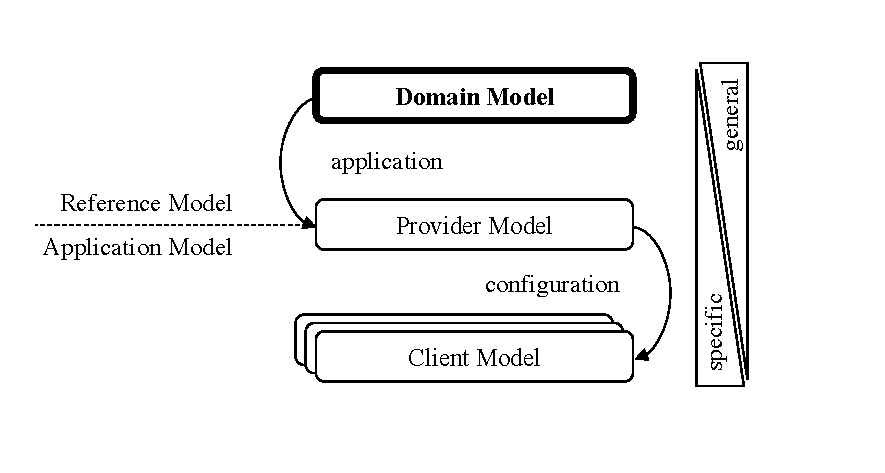
\includegraphics[width=.8\textwidth]{figures/refmodlevels.pdf}}
\end{figure}

The distinction in application and reference model becomes complicated on the provider level. The model is an application of the domain reference model, hence universal validity in the domain vanishes. However, in the domain of the provider this is still valid and has a recommending character as well. With an sufficiently-large client base, diversity of client businesses is captured and therefore the universal applicability is existing to a certain extent. It is noted that sufficiently-large is no further specified here, but Arvato is seen as such a provider\footnote{Arvato is ranked the 6th largest BPO provider 2015 in terms of BPO revenue \citep{hfs2016top}. Explicit numbers for the CRM section of Arvato are not published.}. For this work, the provider model is seen as an application model. Referencing aspects on provider level are considered at construction of the domain level reference model.  

Applying the aforementioned benefits of reference modeling \ref{sec:03_refmod} to the domain in combination with the three stakeholders, one can map these together as in \Tab \ref{tab:refmodbpobenefits}. Therefore it is mandatory to reason the benefits of reference modeling for the different stakeholders in the organization, as design science aims to solve the problem of these parties. The interplay of provider and client model impacts benefits of reference modeling in several aspects and can be attributed mainly to the benefits for Management and Operations.


% Please add the following required packages to your document preamble:
% \usepackage{multirow}
\begin{table}[caption={Benefits of Reference Modelling for BPO-providers in CRM }, label=tab:refmodbpobenefits]
	\centering
	\begin{tabular}{p{1cm} p{2cm} |p{3cm} | p{3cm} | p{3cm} |} 
		\cline{3-5}
		&                                     & \multicolumn{3}{c|}{\textbf{Stakeholder}}                                                                                                                                           \\ \cline{3-5} 
		&                                     & \textbf{Sales}                                          & \textbf{Management}                                 & \textbf{Operations}                                                 \\ \hline
		\multicolumn{1}{|l|}{\multirow{2}{*}{\textbf{Designer}}} & Knowledge                           & \multicolumn{3}{p{3cm}|}{\multirow{2}{*}{\parbox[c]{9cm}{Applicable only to researchers, not to stakeholders in the organization}}}                                                                       \\ \cline{2-2}
		\multicolumn{1}{|l|}{}                                   & Economic benefits from applications & \multicolumn{3}{l|}{}                                                                                                                                                               \\ \hline
		\multicolumn{1}{|l|}{\multirow{5}{*}{\textbf{User}}}     & Cost reduction                      & Faster client approach                                  & Reduced coordination effort                         & More efficient processes                                            \\ \cline{2-5} 
		\multicolumn{1}{|l|}{}                                   & Profit aspects                      & Organized preparation of client meetings                & Standardization facilitates better management       & Usage of new concepts leads to improvement of operational processes \\ \cline{2-5} 
		\multicolumn{1}{|l|}{}                                   & Risk reduction                      & \multicolumn{3}{l|}{\parbox[t]{9cm}{Lower risk of incorrect modeling through reference processes}}                                                                                                  \\ \cline{2-5} 
		\multicolumn{1}{|l|}{}                                   & Analysis                            & Customized offering for approached clients              & Organization-wide benchmarking                     & Benchmarking                                                        \\ \cline{2-5} 
		\multicolumn{1}{|l|}{}                                   & Information Exchange                & Structured communication of value proposition to client & Communication of best practices within organization & Exchange between client operations                                  \\ \hline
	\end{tabular}
\end{table}

BPO is partly cost-driven from a client perspective. For the BPO-provider low costs are therefore a necessity. Cost reduction refers to less effort in coordinating the organization through the used framework and economies of scale and scope across client businesses. For management processes in CRM this means, that a reference process in workforce management enables a more efficient general process on provider level, while on client model level the savings are created. Client-facing processes like sales reduce costs by having a best practice process in the provider model (e.g., run consultative engagements). Operational processes like inbound call handling are always carried out for a specific client and are backbones of the BPO business. While allowing customization in client models, the compatibility to the provider model ensures the connection to reference processes.

Profit aspects often incorporate cost reduction aspects, but stand out through a significant improvement. Realization of up- and cross-selling potentials is one factor, as the necessary steps can be tightly knit into processes. Moreover, historically grown process structures both on client model level and on provider level can be identified. In the CRM domain, improved channel integration through adjusted reference processes benefits both the provider’s abilities towards omni-channel CRM and customer’s perception toward the clients’ customer service, when applied on client model level. As digital channels are becoming the dominant interaction channel, profits through analytics are more in reach.

The analysis aspect expresses the ability to compare and benchmark the business in a new way. Consistent KPI definition enables management to compare across client models, while operations is enabled to improve the analysis of employee performance, as the reference processes cover calculation rules and procedures. As cost efficiency is a primary characteristic in the BPO field, reference modeling supports the provider’s performance management and enables more sophisticated methods through process standardization, especially with respect to more integrated customer service across channels being on the rise.

The last aspect called information exchange phrases the ability \todo{rephrase}to speak a common language in the organization. In the domain of BPO providers this is especially important, because clients vary in their terminology and beliefs of the service. A glossary is seen as an integral part of the reference model to effectively communicate meaning of business vocabulary. As different clients will show different terminology, a consistent management of a general accepted language in the provider’s organization is necessary to ensure comparability. Also, terminology can vary per geographical scope, which adds further complexity and is particularly important for global or multi-national providers. A reference model can propose guidance on this level, while custom definitions in client models will be necessary. Towards client acquisition, the models themselves can be used as basis for discussion, as well as a vehicle to communicate offered services and understanding of CRM.


%

%%%%%%%%%%
\section{DSR Application for Arvato}

 \citeauthor{wilson2002responsible} states that three questions should be asked to research contributions: \enquote{Is it new? Is it true? Is it interesting?} \citep[\p {168}]{wilson2002responsible}. As there is no research found that addresses processes of CRM BPO providers, one can consent the first question. The validity of the artifact, \viz the reference model, is examined on the case at Arvato and aligned with related literature. Regarding the value of this research, one can state the market of BPO amounts approximately 184 billion USD revenue today and CRM services grow above-average \citep{hfs2016top}. As sound processes are critical for both providers and clients. \todo{standardize processes}

\citeauthor{gregor2013positioning} define three levels of design science contribution types, that model the maturity of knowledge in artifacts \citep{gregor2013positioning}. The first level refers to instantiations, \ie situated implementations of an artifact. Level two generalizes by designing constructs, models, that represent knowledge as operational principles or architecture. The highest level positions design theories that hold the most abstract, complete and mature knowledge. 

One research project can build artifacts on multiple levels \citep{gregor2013positioning} and this work aims levels one and two. As the research primarily builds on the case at the research partner Arvato, an instantiation (level one), \viz application in reference modeling terminology, can be undertaken. This serves two purposes. First, it expresses company specifics in comparison to the reference model. Second, it evaluates the use and applicability in a practical use case.  Level two relates to the reference model, that has a higher degree of abstraction. The thesis pursues its construction with priority over the instantiation at Arvato, because there is a unidirectional dependency between the two artifacts: The instantiation has to build on the reference model. The environment in \acrshort{DSR} influences the research and is linked through the relevance cycle. \todo{rephrase}

Following \citeauthor{Hevner2004,Peffers2007}, this work addresses the problem identification and motivation, definition of solution objectives,  design and development. An evaluation is performed based on available information in the exemplary organization and available literature. 


%%%%%%%%%%
%\begin{itemize}%
%	\item wie wende ich DSR hier an?%
%	\item warum wende ich DSR hier an?
%	\item was decke ich mich dieser arbeit ab?
%\end{itemize}

%%%%%%%%%%
\subsection{Problem Identification}
%Activity 1. Problem identification and motivation. Define the specific research problem and justify the value of a solution. Since the problem definition will be used to develop an artifact that can effectively provide a solution, it may be useful to atomize the problem conceptually so that the solution can capture its complexity. Justifying the value of a solution accomplishes two things: it motivates the researcher and the audience of the research to pursue the solution and to accept the results and it helps to understand the reasoning associated with the researcher’s understanding of the problem. Resources required for this activity include knowledge of the state of the problem and the importance of its solution.
CRM is characterized by the components people, process and technology \citep{Chen_2003}, hence BPO outsourcing in this domain needs to address these three components. Here, processes stand in focus.  \cite{schewe2007} see BPO as synthesis of outsourcing and process optimization. The latter necessitates coordination between provider and client, which would benefit from a common basis to build up on. In case of CRM, the distinctiveness of customer contact through the provider adds a challenge that is not typical for BPO in general. 

Diversity in outsourcing contracts require an abstract view on processes, so that the organization can benefit from an appropriate model that enables use of synergies. In case of Arvato CRM, one challenge stems from a decentralized organization, that adds an additional organizational layer which conflicts with company-wide alignment. International clients also demand solutions across countries, which are hard to accomplish without a common understanding. The challenge is rooted in the decentralized internal structure and intensified by complexity of the outsourcing field (\eg, \acrshort{CRM}).

The change to a digital society and with it the increase in contact channels, thereby requiring multi- and omni-channel management, makes an isolated view of channels impractical. \acrshort{IS} need to be designed in order to handle, integrate and make use of diverse channel data for a better customer experience. As BPO providers cannot rely on single systems (\cf \ref{sec:bpocrmis}) which may provide a documented process tailored to the system, a more general representation is needed. Bringing together these aspects formulates a crucial problem for providers and identifies a research gap. 


%wert meiner lösung:
%strukturierung der bpo prozesse.aus unternehmenssicht. grundstein in bpo in crm, aber grundstein für %bpo referenzmodell  
%einführung der levels zur strukturierung der provider / client sichten. erster schritt zu einem bpo %referenzmodell. 
%berücksichtigung von omnichannel crm. 

%%%%%%%%%%
\subsection{Solution Objectives}
%anforderungsdefinitionen nach püster
%der kasten: thomas 248, vombrocke 98, püster 63, 

%%%%%%%%%%
%Activity 2. Define the objectives for a solution. Infer the objectives of a solution from the problem definition and knowledge of what is possible and feasible. The objectives can be quantitative, e.g., terms in which a desirable solution would be better than current ones, or qualitative, e.g., a description of how a new artifact is expected to support solutions to problems not hitherto addressed. The objectives should be inferred rationally from the problem specification. Resources required for this include knowledge of the state of problems and current solutions, if any, and their efficacy.

Based on identified problems, solution objectives outline requirements, that the reference model artifact should contain. A morphological box helps to structure reference model attributes. This pattern draws from the work of \cite{Puster2015} and \textbf{highlights} pursued characteristics in \Tab \ref{tab:morph}.  

\begin{table}[caption={Reference model requirements }, label=tab:morph]
	\centering
		\begin{tabular}{ 
				p{3.1cm}  
			p{2cm} p{2cm} p{2cm} p{2cm} p{2cm} p{2cm} p{2cm} p{2cm} p{2cm} p{2cm} p{2cm} p{2cm}    }
			Attribute                                   & \multicolumn{12}{c}{ Characteristic }                                                                                                                  \\ \hline
			\multicolumn{1}{|l|}{\textit{Reusability}}          & \multicolumn{6}{c|}{\textbf{generic reference model}}                       & \multicolumn{6}{c|}{non-generic reference model}                  \\ \hline
			\multicolumn{1}{|l|}{\textit{Purpose}}              & \multicolumn{6}{c|}{\textbf{organizational design}}                         & \multicolumn{6}{c|}{application system design}                    \\ \hline
			\multicolumn{1}{|l|}{\textit{Description level}}    & \multicolumn{4}{c|}{\textbf{concept}}                & \multicolumn{4}{c|}{data processing concept} & \multicolumn{4}{c|}{implementation}       \\ \hline
			\multicolumn{1}{|l|}{\textit{Description type}}     & \multicolumn{4}{c|}{\textbf{As-Is}}                  & \multicolumn{4}{c|}{To-Be}                   & \multicolumn{4}{c|}{Ideal}                \\ \hline
			\multicolumn{1}{|l|}{\textit{View}}                 & \multicolumn{3}{c|}{organization} & \multicolumn{3}{c|}{data}    & \multicolumn{3}{c|}{functions}   & \multicolumn{3}{c|}{\textbf{process}} \\ \hline
			\multicolumn{1}{|l|}{\textit{Knowledge generation}} & \multicolumn{6}{c|}{\textbf{induction}}                                     & \multicolumn{6}{c|}{\textbf{deduction}}                                    \\ \hline 
			\multicolumn{13}{r}{Adapted from: \citep[\p{63}]{Puster2015},\citep[\p{98}]{brocke2003referenzmodellierung}, \citep[\p{248}]{thomas2006mang}  }       
			
	\end{tabular}
\end{table}

In terms of reuseability, the reference model is intended to be generic, so that it is reusable for a class of companies. Here, these are providers of business process outsourcing in customer relationship management. With the previously discussed provider models, one can name a non-generic reference model. Distinguishing processes of the domain are prioritized in the construction, as their value contribution to the model is higher in comparison to generic processes, that do not differ significantly from other domains (accounting for instance).  

The purpose of the model is seen in organizational design. Drawing on the listing of use cases given by \cite{Rosemann2012proc}, knowledge management and organizational documentation can be named in the first place. 

The \acrshort{ARIS} introduces three different conceptual levels with increasing IT-orientation. The reference model is seen on concept level, which facilitates comfortable communication with the business. 
\todo{+++}

Regarding the description type, one can separate into three three model orientations. As-is aims to describe the current state of the domain, \viz showing common practices. To-be models a future state that incorporates wanted changes. \todo{ideal?} Ideal modeling displays an optimal scenario. In this case, the intention is to capture the current state of the domain. 

The process view integrates the organizational, data and functional perspective. It is noted that the time-logical sequence of processes may be of subordinate importance, as an application probably causes reordering of process steps. Nevertheless, the process view is the medium for capturing aspects from other perspectives, while leaving room for individual adjustments without sacrificing model integrity. 

As mentioned before, induction and deduction are employed for knowledge generation.
 
\subsubsection{General objectives}
Combining these attributes implies demands, that relate to the solution objectives.

\hfill\begin{minipage}{\dimexpr\textwidth-1.2cm}
	\textbf{Solution Objective 1}: Construction of a generic  reference model that covers distinguishing processes for BPO-providers in CRM on concept level
	\\
	
	\textbf{Solution Objective 2}: The reference model can be applied for use at Arvato CRM.  
	\\
	
	\textbf{Solution Objective 3}: The construction  process is well-documented, makes use of empirical research by induction, which is enriched by deduction from \acrshort{BPO} and \acrshort{CRM} theory.
	
	\xdef\tpd{\the\prevdepth}
\end{minipage}

The choice of the modeling language should not interfere with the intended use in the industry. As no studies regarding process modeling language use are available to the best knowledge of the author, the language should be transferable into popular candidates, \eg \acrshort{BPMN} and \acrshort{EPC}. For reference modeling as such, there is neither a standard existing, but a trend towards use of existing languages exists \citep{Fettke2004}. 

While reference models aim for content-wise standardization, the use of formalized languages helps to sustain syntactic and semantic quality in the model \citep{Fettke2004}. By doing this, the model should be comprehensible with ease from members of the business and IT organization. 

\hfill\begin{minipage}{\dimexpr\textwidth-1.2cm}
	\textbf{Solution Objective 4}: A syntactic and semantic formalized process modeling language is used, that is transferable to other languages. 
	
\end{minipage}

\subsubsection{Stakeholder-related objectives}

Building on the discussion in \ref{sec:refmodusearvato}, the benefits of reference modeling in the domain are stated. Putting objectives of this work in direct relation to the three identified stakeholders is difficult, as the model represents the whole provider organization. The overall goal of increased alignment reasoned the decision to create this model at the research partner on a board level. However, the stakeholder's benefits do not directly create objectives. The construction merely should consider realization of the identified benefits, by incorporating requirements for their realization.  Consequently, these requirements are formulated as objectives.  

The organization uses an application model (provider model) that draws from the reference model, which is discussed in this work. Hence, stakeholder-related objectives are motivated by an application model and then mirrored towards the reference model. In this regard, the following paragraph uses the term model to express this ambiguity. 

Sales is oriented towards clients and the model is a means to communicate more effectively with them. Their interest externally lies in a use as a statement of competence. The management uses it to encompass idiosyncrasies across client businesses. Thereby it facilitates alignment, which is incorporated in the use of reference models for organizational design (\cf \Tab \ref{tab:morph}). Operations is supported by the model to handle complexity of increasing channels and benefits from reference processes, as they enable standardized approaches. \todo{+++}
\\

\hfill\begin{minipage}{\dimexpr\textwidth-1.2cm}
	\textbf{Solution Objective 5}: The model can be used as a statement of competence for sales activities towards clients.
	\\
	
	\textbf{Solution Objective 6}: The model holds a process representation, which supports a common understanding across client businesses. 
	\\
	
	\textbf{Solution Objective 7}: The model is able to represent an omni-channel environment. 

\end{minipage}


\section{Limitiations}
%%%%%%%%%%

The title of this thesis expresses limitations in two ways. Firstly, its research is \textit{towards} a reference model. It is not intended to complete the model with this work. It lays a foundation for detailed investigation in its components. Processes are only partly described on the lowest detail level. Also the focus is set on distinguishing processes in the domain, which neglects support processes as defined in \ref{processorientation}. The simplification in this thesis can be justified by the fact that the contribution to the knowledge base is insignificant for support processes, as these are subject to publications beyond number. 

Secondly, \textit{a reference model} is meant, which signifies limitations in used data to construct the model. As the primary data source the research partner and its organization as an example of a BPO provider in CRM, one can object the dispensation of an investigation in other providers. However, due to the nature of the BPO business with multiple client businesses and the size of the research partner, diversity is captured to a certain extent. 

While the process view includes aspects of the data, organizational and functional perspective, especially a dedicated data view would be beneficial to out research in an omni-channel environment. The integration of data to identify customers across channels is an important, yet unsatisfactory explored research area. In this regard the process reference model helps to convey a perspective of activities from a time-logical order, to identify and structure moments that are important \wrt data availability, access or creation. 

Regarding the structure of domain, provider and client model, it is noted that this proposal is only outlined in this work and not further described through generic reference modeling techniques, as discussed in \cite{delfmann2006adaptive, brocke2003referenzmodellierung}. 

The thesis puts special emphasis of customer service processes (\cf \ref{sec:crm},  \Fig \ref{fig:crmprocessfr}). Outsourcing operational \acrshort{CRM} may also be leaned towards other operational processes of CRM, like marketing or sales. However, customer service is the most frequent case, while clear boundaries vanish. This reasons the framing of the reference model in \acrshort{CRM} instead of customer service. 

%\begin{itemize}
%	\item only core processes specified, as also done in retail-h ok
	%\item core processes partly on lowest level
%	\item process refmod, not data,...
%	\item provider, client model construct only outlined 
%	\item specified later
	%	\item one company
%\end{itemize}
%%%%%%%%%%

